\section{System Architecture}
\label{sec:arch}
\system{} links team coordination to plant interaction through industrial nodes
and production context (Fig.~\ref{fig:arch}). Channels coordinate deployed
members and tasks; controller services mediate node operations; production
objects identify the line, product, recipe, and run. Five planes separate the
concerns: a \emph{team} plane decides what to investigate and propose, an
\emph{integration} plane presents devices as semantic nodes, a \emph{governance}
plane decides whether a request is admissible, an \emph{operations} plane
supplies production context and evidence, and an \emph{extensibility} plane
admits drivers and services through sanctioned registration points. The
decomposition is what makes the framework reusable: scenario knowledge sits in
blueprints, signal maps, predicates, and driver configuration, not in team
scheduler, approval service, or persistence code.

\begin{figure*}[!t]
\centering
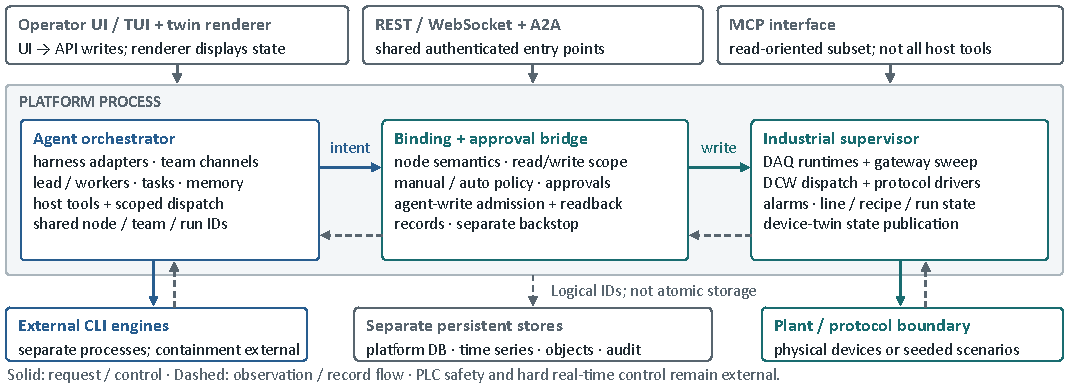
\includegraphics[width=\textwidth]{resources/fig2-architecture.pdf}
\caption{System architecture and execution boundaries. The platform hosts team
routing, binding and approval, industrial supervision, and records. Operator
interfaces sit above it; agent engines, data stores, protocol endpoints, and
the plant remain separate. Shared identifiers provide attribution but do not
make storage and actuation transactional.}
\label{fig:arch}
\end{figure*}

Each plane draws its own boundary between platform guarantees and scenario
inputs: team coordination owns member identity, task state, and a
member-written episodic memory retrieved by hybrid search; industrial
integration owns protocol acceptance, readback, freshness, and transport
errors, its node stream feeding both the agent and a live digital-twin view;
governance owns admission, approval, actuation, write readback, observation,
verdict, compensation, and rollback; production operations attaches line,
product, recipe, and run context while PLC protection stays independent; and
extensibility admits plugins, drivers, agent tools, panels, and SDK clients
through sanctioned services. In every plane the common execution path is
unchanged: what a scenario supplies is data and strategy.

\subsection{Supervisory Core and Nodes}
The Node.js core hosts channel routing, industrial services, and protocol
adapters. A channel contains a lead, workers, tasks, messages, and retrievable
memory, deployed through WebSocket, MCP, A2A, REST, CLI, or TUI entry points; engine adapters preserve
member and node identity across runtimes, and channel membership alone confers
no write authority.

DAQ nodes convert device readings to engineering quantities; DCW nodes translate
engineering setpoints into driver commands and, where supported, readback.
Per-node runtimes manage timing; gateway services supply
connection state, recipe context, and write bookkeeping. The built-in semantic
surface covers Modbus TCP, Modbus RTU-over-TCP, OPC UA, MQTT, and HTTP/REST as
both client and server endpoints, plus S7 for acquisition only.
The deployment reaches author-implemented dynamic simulators through the same
node and driver contracts a plant would use; they are deterministic per seed
but not validated digital twins. The first reuse boundary is declarative: a
scenario declares signals, units, scaling, precision, and driver
configuration, and the team loop is unchanged; fast regulation and independent
protection stay in plant controllers.

Driver contracts are deliberately narrow: a driver declares how a semantic
quantity maps to its transport payload, whether the endpoint is writable, and
whether a readback is available, while the controller resolves member authority
and active limits. Connection, transport, and protocol errors attach to the
request rather than one success flag, and register addresses and byte order
appear only here, so a new fieldbus family leaves the loop untouched.

Acquisition is supervisory rather than hard real-time: each DAQ node runs its
own cadence under a rotating sweep, so a slow endpoint delays only its own
samples. The verdict stage queries the timestamped, quality-stamped history
rather than issuing a blocking read, which is why a windowed average can lag
the device by one cadence.

\subsection{Bindings, Context, and Reuse Boundaries}
A member--node binding grants access to a sanctioned tool on a specific node and
selects automatic or approval-mediated execution. Line permissions (none,
read-only, operate) authorize binding creation and mutation; runtime
invocation is authorized by the persisted capability, not channel membership.
Intervals are re-checked every request instead of cached, so revoking
a binding or switching the recipe takes effect on the next request. The same path
serves a console, a harness, and an agent engine, because authority does not
depend on the client; only the evidence record differs.

Production objects are versioned rather than overwritten: a recipe is dispatched
against a known-good version, reverted non-destructively, and compared with the
values actually applied, and an intervention is read against the definition
that was active when it was admitted. Plugins register hooks, routes, agent tools, drivers,
and panels only through sanctioned services, so an added driver inherits
admission, readback, and evidence capture. A BOPET worker proposes casting-speed,
fast-roll, or rail-width changes through bound DCW nodes, and the same mission
pattern serves the other three scenarios with only blueprint, guards, and policy
differing (Section~\ref{sec:scenarios}).

The second reuse boundary is a reference scenario-onboarding adapter
(Section~\ref{sec:onboarding}); the SDK exposes the same surface to ordinary
programs, and runtime settings are hot-reloadable. The stores share identifiers
rather than a transaction domain: platform state uses SQLite and files, and
measurement and object backends use TimescaleDB and MinIO with local fallbacks.
A device may accept a write even if bookkeeping fails, and records lack a run
identifier, so time-range queries can cross runs unless bounded.

\subsection{Reference Scenario-Onboarding Contract}
\label{sec:onboarding}
The reference integration follows a bounded onboarding contract: the engineer
declares a blueprint of devices, signals, units, roles, setpoints, and
plant-model parameters; a differential ``ensure'' pass creates missing
devices, repairs drift, verifies connectivity, loads the model without
disturbing other lines, projects the blueprint into semantic nodes and a
recipe, and tags the line for idempotent reuse; a channel is built from the
common team template with the required bindings; and a mission supplies
objective, guards, response windows, and policy. The adapter demonstrates reuse
of platform services, not configuration-only commissioning of physical plants.

\subsection{Governed Optimization Task Life Cycle}
\label{sec:tasklifecycle}
A governed optimization task is a life cycle rather than a single tool call, and
\system{} exposes each transition separately. The task enters a channel carrying
goal, line, product, recipe, run, and task identifiers; a lead member claims it
and hands it to a worker holding member--node bindings on the relevant nodes.
The worker then repeats one fixed job: read the controlled quantity over a
bounded window, propose a setpoint inside the resolved interval, invoke the
governed write, wait for the response, and record a verdict
(Section~\ref{sec:procedure} instruments it).

Each iteration therefore leaves more than a written value: the write opens an
optimization record carrying prior and requested values, the admitting
interval, the acting member, and timestamps; readback, where supported, closes
the command path; the parameter journal attributes the change to its source; and
attainment is computed against the scenario predicate while the task closes with
a workflow terminal state. This bounds what ``automatic optimization'' means
here: a
controller, a scripted policy, a conventional optimizer, or an agent engine may
occupy the strategy slot, while authority, evidence, and closure stay on the
platform---and a mission may reach its terminal state while missing the process
objective, because the two are never merged.
